% Copyright Patrick Hall 2019
% CC by 4.0 license

\documentclass[fleqn]{article}

\renewcommand\refname{}

\title{On Unhelpful Explainable Machine Learning Misconceptions}

\author{
  Patrick Hall\footnote{H2O.ai and George Washington University} \footnote{\copyright \hspace{1pt} Patrick Hall 2019. This work in progress is shared under a CC by 4.0 license.}\\
  Washington, DC\\
  \texttt{patrick.hall@h2o.ai}
}

\usepackage{graphicx}
\usepackage{fullpage}
\usepackage{pdfpages}
\usepackage{amsmath}
\usepackage{amssymb}
\usepackage{mathtools}
\usepackage{MnSymbol}
\usepackage{enumerate}
\usepackage{setspace}
\usepackage[colorlinks]{hyperref}
\usepackage{breakurl}
\usepackage{float}
\usepackage{caption}
\usepackage{subcaption}
\usepackage{multicol}
\usepackage{color}
\usepackage{listings}
\usepackage{csvsimple}
\usepackage{algorithm}
\usepackage{algorithmic}
\usepackage{verbatim}
\usepackage{mdframed}
\usepackage{changepage}
\usepackage[top=1in, bottom=1in, left=1in, right=1in]{geometry}

\begin{document}

\maketitle

\begin{abstract}

This short text presents arguments, proposals, and references to address recently uncovered misinformation and misconceptions about explainable machine learning. It also argues that post-hoc explanatory methods are one of several viable types of tools in a holistic, human-centered, and low-risk approach to machine learning.

\end{abstract}

\section*{Introduction}

``Please stop doing explainable machine learning,'' extolled one of the brightest minds in machine learning (ML) with the title of a recent and well-reasoned essay \cite{please_stop}. A related and admittedly-controversial short talk also included points such as, ``[Explainable ML] forces you to rely on two models instead of one,'' and argued that explainable machine learning can be a foil for companies and governments to conduct unsavory or negligent deeds with black-box models.\footnote{Statistics at a Crossroads, Webinar 2. URL: \url{https://zoom.us/recording/play/0y-iI9HamgyDzzP2k_jiTu6jB7JgVVXnjWZKDMbnyRTn3FsxTDZy6Wkrj3_ekx4J?startTime=1538497702000}} Perhaps even more noteworthy was the online response, which included musings such as, ``don’t forget hidden assumptions for explainable ML (e.g., locally linear behavior near predictions),'' and lamentations like, ``no one has explained to me what 'explainable' or 'interpretable' is.'' \footnote{Twitter thread: \url{https://twitter.com/tdietterich/status/1052680788389507073}} This article aims to clear up such misconceptions and fill the gaps in community knowledge exposed by these sentiments.

%Strangely, neither the talk nor the follow-up discussions seemed to allow for combining white-box models and post-hoc explanatory techniques. 

\begin{figure}[htb]
	\begin{center}
		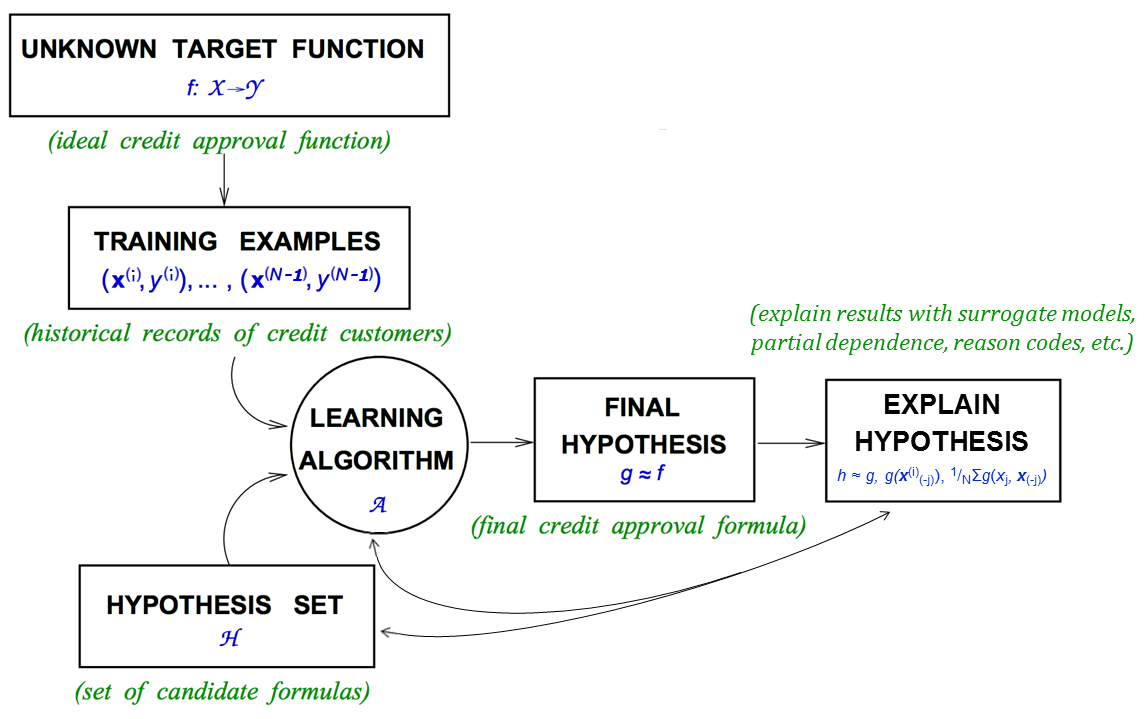
\includegraphics[scale=0.33]{img/figure_1.png}
		\caption{An augmented learning problem diagram in which several post-hoc techniques create explanations for a credit scoring model $g$. When used properly, explanations can increase understanding of $g$ and help improve the accuracy, fairness, interpretability, privacy, or security of subsequent applications of $\mathcal{H}$ and $\mathcal{A}$. Adapted from Figure 1.2 of the open textbook \textit{Learning From Data} \cite{lfd}.}
		\label{fig:learning_problem}
	\end{center}
\end{figure}	

To avoid ambiguity, and as illustrated in Figure \ref{fig:learning_problem}, here explainable ML means post-hoc techniques used to understand trained model behavior or predictions. Examples of common explainable ML techniques include:

\begin{itemize}
\item Local and global feature importance methods, in particular Shapley values \cite{shapley1988shapley}, \cite{keinan2004fair}, \cite{kononenko2010efficient}, \cite{shapley}.
\item Local and global model-agnostic surrogate models, such as surrogate decision trees and Local Interpretable Model-agnostic Explanations (LIME) \cite{dt_surrogate1}, \cite{dt_surrogate2}, \cite{lime-sup}, \cite{lime}. 
\item Local and global visualizations of model predictions such as 1- and 2-dimensional partial dependence and individual conditional expectation (ICE) plots \cite{esl}, \cite{ice_plots}.
\end{itemize}  

By presenting clarifications, highlighting definitions, and addressing misconceptions, this text also builds a seemingly natural case for a holistic approach to ML that includes white-box models along with explanatory and disparate impact analysis and remediation techniques.  %The article also implies that ignoring an entire set of methods because \textit{some subset} of the methods are approximate is akin to throwing the baby out with the bath water. 
\textbf{This text does not condone the use of black-box models without explanation and disparate impact analysis.} That practice is now outdated, likely lazy and unethical, and potentially dangerous.

\section{Misconception: Explanations are Necessary and Sufficient to Establish Trust in ML}

Explanations are likely necessary for trust in many cases, but certainly not sufficient for trust in all cases. 
Explanation, as a general concept, is related more directly to understanding and transparency than to trust.\footnote{The Merriam-Webster definition of \textit{explain}, accessed April 21\textsuperscript{st} 2019, does not mention \textit{trust}} Simply put, one can understand and explain something without trusting it. One can also trust something and not be able to understand or explain it. Consider the following example scenarios:

\begin{itemize}

\item \textbf{Explanation and understanding without trust}: After a disparate impact and explanatory analysis, a practitioner finds substantial errors or demographic disparity in model predictions or they find counter-intuitive or hackable attributes in the model's decision-making mechanisms. In this example scenario, the model is explainable and well-understood, but not trustworthy. 

\item \textbf{Trust without explanation and understanding}: Years before reliable explanation techniques were widely acknowledged and available, black-box predictive models such as neural networks were used for fraud detection in the financial services industry \cite{gopinathan1998fraud}. When these models performed well, they were trusted.\footnote{For example: \url{https://www.sas.com/en_ph/customers/hsbc.html}.} However, they were not explainable or well-understood by contemporary standards.  

\end{itemize}

If trust in models is your goal, then explanations alone are not sufficient. However, as discussed in Section \ref{sec:white_box} and illustrated in Figure \ref{fig:hc_ml}, in an ideal scenario, explanation and understanding would lead to better accuracy, fairness, interpretability, privacy, security, and trust in ML models. (In this text, \textit{fairness} refers to observational fairness as quantified by disparate impact analysis.)

\section{Misconception: Explainable ML is Unnecessary}

Explanation of model mechanisms and predictions is mandated under the Fair Credit Reporting Act for credit lending decisions. Explanation, along with disparate impact analysis and the documentation they enable, can also be required under the Civil Rights Acts of 1964 and 1991, the Americans with Disabilities Act, the Genetic Information Nondiscrimination Act, the Health Insurance Portability and Accountability Act, the Equal Credit Opportunity Act, the Fair Housing Act, Federal Reserve SR 11-7, the European Union (EU) Greater Data Privacy Regulation (GDPR) Article 22, and other regulatory statutes \cite{ff_interpretability}.

\section{Misconception: All the Key Terms in Explainable ML are Undefined}

Helpful definitions that apply to explainable ML have been put forward, including:

\begin{itemize}
\item \textbf{Interpretable}: ``The ability to explain or to present in understandable terms to a human'' -- in ``Towards a Rigorous Science of Interpretable Machine Learning'' by Doshi-Velez and Kim (2017) \cite{been_kim1}.
\item \textbf{A Good Explanation}: ``When you can no longer keep asking why'' -- in ``Explaining Explanations: An Approach to Evaluating Interpretability of Machine Learning'' by Gilpin et al. (2018) \cite{gilpin2018explaining}. (Gilpin et al. also provide several clear constructs for describing more specific types of explanations.) 
\end{itemize}



While the explainable ML field is far from embracing a clear and accepted taxonomy of concepts or an exhaustive and precise vocabulary, these two well-founded definitions appear to link explanations to some ML process being interpretable. Moreover, many authors have made significant attempts to grapple with a variety of general concepts related to interpretability and explanations, including ``A Survey Of Methods For Explaining Black Box Models'' by Guidotti et al. (2018), Zachary Lipton's ``The Mythos of Model Interpretability'' (2016), Christoph Molnar's \textit{Interpretable Machine Learning} (2018), and Adrian Weller's ``Challenges for Transparency'' (2017) \cite{guidotti2018survey},  \cite{lipton1}, \cite{molnar}, \cite{weller2017challenges}. 

\section{Misconception: Explainable ML is Just Models of Models}

Models of models, or surrogate models, can be helpful explanatory tools, but they are usually approximate, low-fidelity explainers. Aside from 1.) a global summary of a complex model provided by a surrogate model can be helpful sometimes and 2.) much work in explainable ML has been directed toward improving the fidelity and usefulness of surrogate models \cite{dt_surrogate1}, \cite{dt_surrogate2}, \cite{lime-sup}, \cite{wf_xnn}, \textbf{many explainable ML techniques have nothing to do with surrogate models!}   

One of the most exciting breakthroughs for supervised learning problems in explainable ML is the application of a coalitional game theory concept, Shapley values, to compute feature contributions which are consistent globally and accurate locally using the trained model itself \cite{kononenko2010efficient}, \cite{shapley}. An extension of this idea, called tree SHAP, has already been implemented for popular tree ensemble methods \cite{tree_shap}. There are many other explainable ML methods that operate on trained models directly such as partial dependence and ICE plots \cite{esl}, \cite{ice_plots}. Notably, surrogate models and explanatory techniques that operate directly on trained models can be combined, for instance by using partial dependence, ICE, and surrogate decision trees to investigate and confirm modeled interactions \cite{art_and_sci}. 

For a curated list of many different types of white-box modeling techniques, and model-specific, model-agnostic, and surrogate model explainable ML techniques, please see:
\begin{center}
\url{https://github.com/jphall663/awesome-machine-learning-interpretability}
\end{center}

\textbf{Misconception Corollary: Explainable ML is just LIME.} LIME, in it's most popular implementation, uses local linear surrogate models \cite{lime}. LIME is important, and imperfect, but just one of many explainable ML tools. And again, LIME can sometimes be combined with model-specific methods to yield deeper insights. Consider that tree SHAP can provide locally accurate and consistent point estimates for local feature importance whereas LIME can provide approximate information about modeled local linear trends around the same point.   

\section{Misconception: Explainable ML Methods Simply Provide Cover to Use Black-Box ML for Nefarious Purposes}

If used disingenuously, explainable ML methods probably do provide such cover \cite{fair_washing}. But explainable ML methods were designed specifically to crack open those same nefarious and complex black-boxes. See Angwin et al. (2016) for evidence that hacking or stealing of commercial black-box models for oversight purposes is possible \cite{angwin16}. Such investigations would likely only be improved by advances in explanatory and fairness tools. Additionally, many important computer-based technological advances present similar double-edged sword dilemmas, e.g. social media or strong encryption. Rarely does the ability of a tool to be misused for malicious purposes disqualify it from being used as designed. 

\section{Misconception: Explainable ML Methods and White-box Models are Somehow Mutually Exclusive} \label{sec:white_box}

A few well-known publications have focused either on white-box modeling techniques (e.g. \cite{slim}, \cite{sbrl}) or on post-hoc explanations (e.g. \cite{lime}, \cite{shapley}), but the two can be used together in the context of a broader and more human-centered machine learning workflow as illustrated in Figure \ref{fig:hc_ml}. 

\begin{figure}[htb]
	\begin{center}
		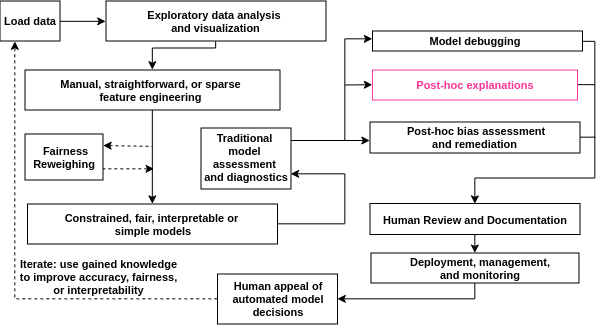
\includegraphics[scale=0.15]{img/figure_2.png}
		\caption{A diagram of a proposed human-centered machine learning workflow in which explanations (highlighted in green) are used along with interpretable models, disparate impact analysis and remediation techniques, and other review and appeal mechanisms to create a fair, accountable, and transparent ML system.}
		\label{fig:hc_ml}
	\end{center}
\end{figure}	

Consider the seemingly useful example case of augmenting globally interpretable models with local post-hoc explanations: A practitioner could train a single pruned decision tree as a globally interpretable model then use local explanations in the form of Shapley feature importance. This would enable the practitioner to see accurate numeric feature contributions for each model prediction in addition to the entire directed graph of the decision tree. Isn't a complete global and local understanding of the model more desirable than the white-box model or the post-hoc explanations alone?\\ 

\textbf{Corollary Misconception: Explainable ML Methods and Fairness Methods are Somehow Mutually Exclusive}: Like white-box models, fairness methods are often presented in different articles than post-hoc explanatory methods. However, in banks, using post-hoc explanatory tools such as partial dependence plots and local feature importance to comply with credit reporting regulations often goes hand-in-hand with using disparate impact analysis to comply with fair lending regulations. 

\section*{Conclusion}

This short text is not an attack on any party. However, it does promote informed debate, scrutiny, and development of explainable ML, and not the dismissal or derision the discipline. Explainable ML methods have already been implemented into popular open source software and into commercial software.\footnote{Like h2o-3, xgboost, and various other Python and R packages. See: \url{https://github.com/jphall663/awesome-machine-learning-interpretability} for a longer, curated list of open source software packages.}\textsuperscript{,}\footnote{At least Datarobot, H2O Driverless AI, SAS Visual Data Mining and Machine Learning, Zest AutoML as of April 21\textsuperscript{st} 2019} They will likely be used widely. Proper usage discussions are likely more practical than ``please stop'' requests. Moreover, much credible work has been done in several disciplines to make machine learning more interpretable and trustworthy, and thus better as a science. All of that work is likely less valuable in silos, and likely more valuable and practical when used in combination. As argued in this short text, the proper usage of explainable ML today appears to be along side of interpretable models and disparate impact analysis. 

\section*{Acknowledgemnts}

The author thanks Pramit Choudhary and Navdeep Gill at H2O.ai for their input and insights. 

%-------------------------------------------------------------------------------
\section*{References}
%-------------------------------------------------------------------------------
\bibliographystyle{plain}
\bibliography{xai_misconceptions}

\end{document}

% let doug proofread